\chapter{Introduction}
		\section{Objectif général du projet}
		\paragraph{Quel est le problème à régler?}
		Dans un jeu de Tron dont les règles sont explicitées dans la partie sur le modèle, nous allons faire jouer deux équipes:
		
		\begin{itemize}
			\item Un joueur seul et intelligent
			\item Une coalition de joueurs moins intelligents
		\end{itemize}
		
		Le but est d'analyser les meilleurs paramètres pour que notre coalition soit statistiquement la plus efficace contre le joueur seul, si une tendance se dégage de nos simulations.
		
		En d'autres termes, nous allons tenter de répondre à la question:
		
		
		\begin{problem}
			\sffamily
			Combien faut-il d'idiots pour prendre l'avantage sur un joueur plus intelligent?
		\end{problem}
	
		\section{Objectifs à atteindre}
		\paragraph{Simulateur} 
		Une interface permettant de suivre la progression de la simulation est très importante pour estimer quand terminent nos simulations.
		
		\paragraph{Modèle de jeu}
		Le moteur de jeu devra être le plus optimisé possible pour éviter de couter en temps de simulation pour l'heuristique et permettre le calcul d'un maximum de parties.
		
		\paragraph{IA et son heuristique}
		L'intelligence artificielle va devoir être capable de se défendre et d'attaquer l'équipe adverse de façon efficace et l'heuristique devra être optimisée au possible.
		
		\paragraph{Stockage de masse}
		Au vu des grandes quantités de données potentielles, une base de donnée bien structurée avec des vues permettant de faciliter l accès aux informations pertinentes pour l'analyse sera primordiale.
		
		\paragraph{Analyse statistique}
		Nous allons devoir faciliter la visualisation et le travail sur nos données afin de permettre de se concentrer sur l'analyse plutôt que sur les outils d'analyse. Il sera donc important d'unifier au possible les moyens d'analyse des données et de rédaction d'analyses pour augmenter notre efficacité.
		
		
		\part{Cahier des charges}
		

		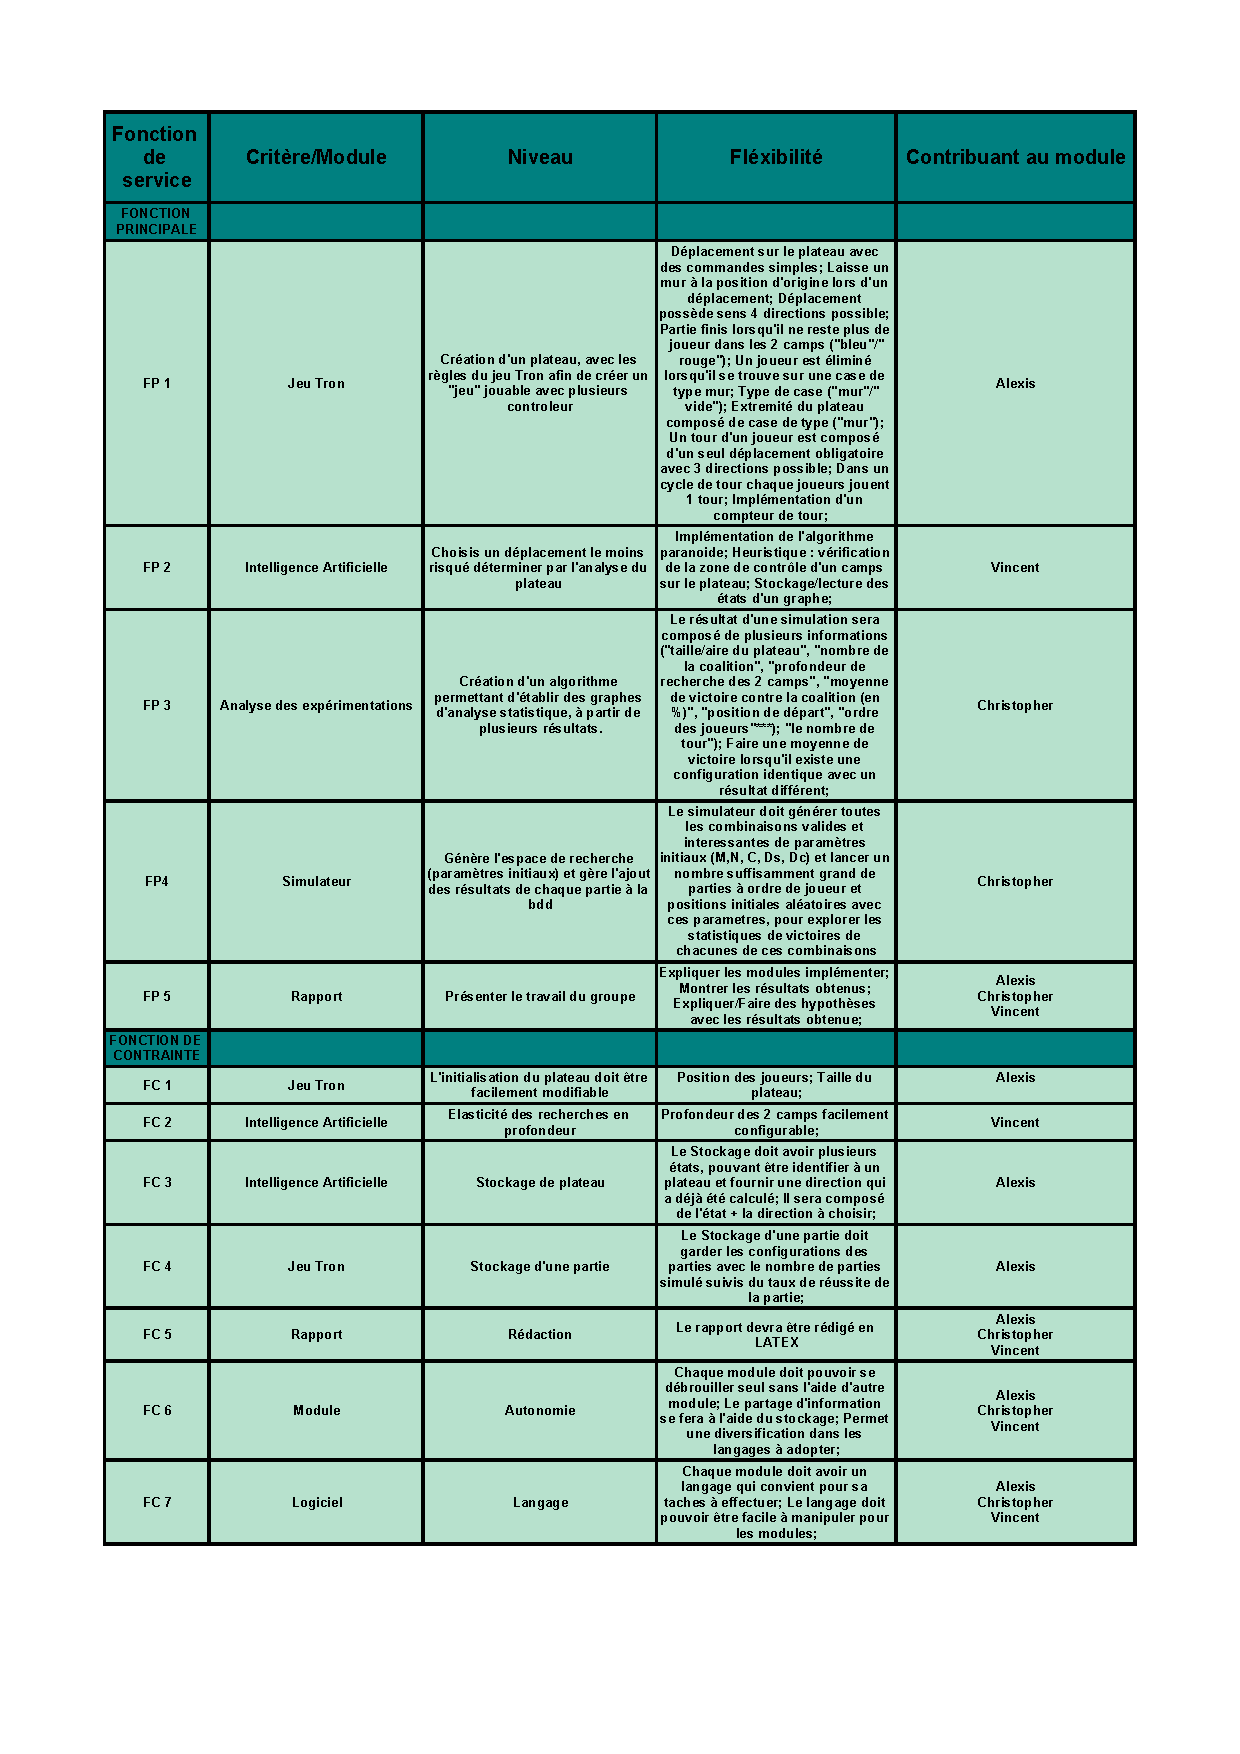
\includepdf[pages=-]{./data/cahier.pdf}
		
		\section{Spécifications}
			\subsection{Spécification des paramètres de simulation}
				
				\begin{figure}[H]
					\centering
					\begin{tabular}{l l}
						Paramètre de simulation&Signification\\\hline
						M & Longueur du terrain\\
						N & Largeur du terrain\\
						C & Nombre de joueurs dans la coalition\\
						Ds & Intelligence du joueur solo\\
						Dc & Intelligence des joueurs de la coalition
					\end{tabular}
					\caption{Nomenclature des paramètres de jeu}				
				\end{figure}
				
			\subsection{Contraintes techniques}
				\paragraph{Temps imparti réduit}
				
				Suite à une annulation de la matière puis à la réouverture de celle ci, le temps imparti pour ce projet as été considérablement amoindri.
				
				Nous avons environ 5 semaines pour mener ce projet à terme à compter du 31 janvier 2019.
				Il est donc nécessaire de réduire un maximum les temps de développement pour le mener à bien.
				
				Cela a mené à la nécessité d'évaluer nos options de façon la plus pragmatique possible en termes de coûts en temps d'implémentation.
				
				
				
		
		\section{Choix techniques}
			\subsection{Architecture}
			\img{./pics/archi}
			
			\subsection{Langages utilisés}
			
			
				\paragraph{Module simulation:}
				\begin{itemize}
					\item Python pour l'interface commande et les sous modules internes.
					\item SQL pour la génération et l'interaction avec la bdd
				\end{itemize} 
				
				
				\paragraph{Module analyse:}
				\begin{itemize}
					\item R pour la génération des graphes et la manipulation des données
					\item Markdown pour la rédaction du rapport d'analyse
				\end{itemize}
			
			\subsection{Accès au code source}
			Vous pouvez trouver \href{https://github.com/helldragger/PolTron-La-coalition}{
			\bfseries \color{link} l'intégralité du code source ici.}
		\part{Historique des travaux réalisés}
		
		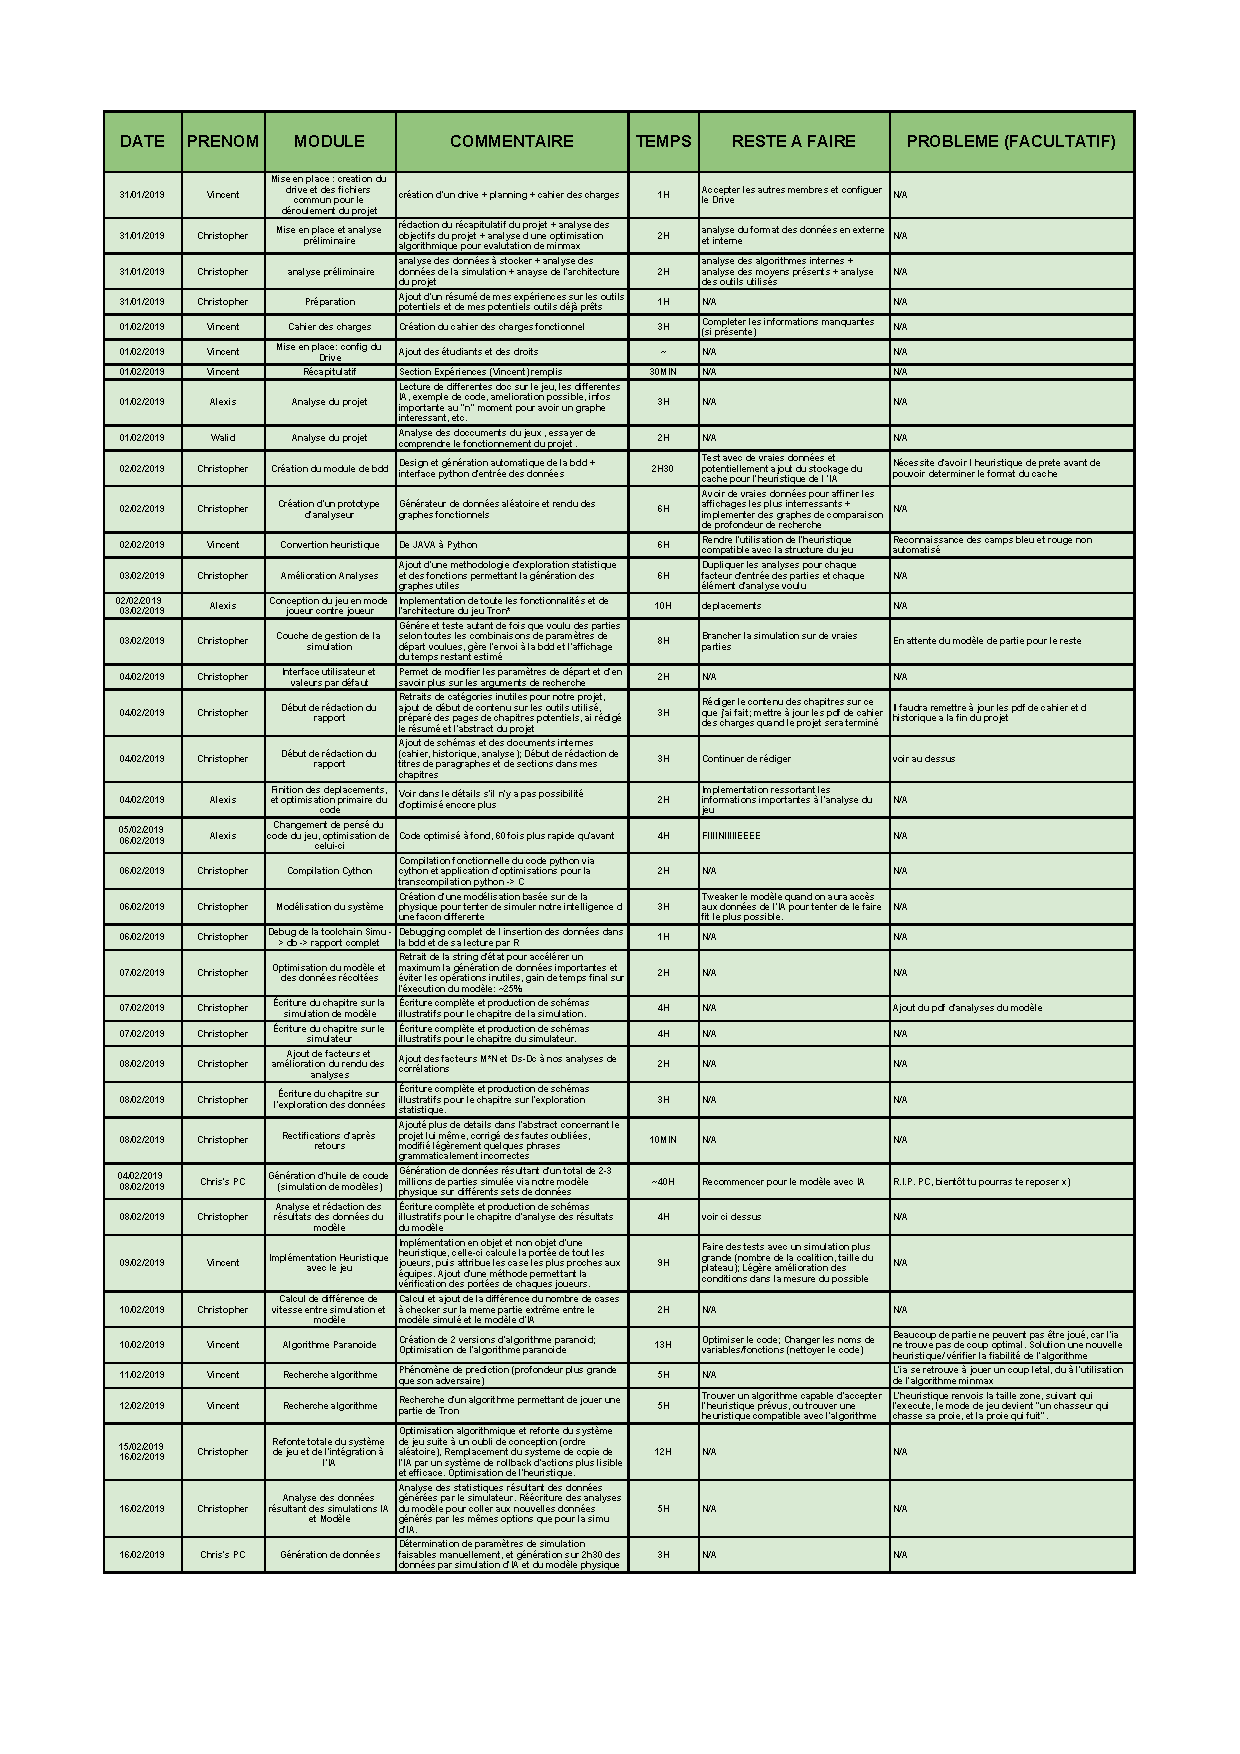
\includepdf[pages=-]{./data/historique.pdf}
		% etc...
		\paragraph{Concernant Walid}
		
		Suite à une discussion sur les expériences, et compétences de chacuns pour analyser comment mener au mieux ce projet, un accord a été passé avec Walid pour qu'il puisse se familiariser de son côté avec Python et aux concepts du projets en tentant d'en réaliser un maximum de son coté.
		
		Afin de ne pas le délaisser non plus, il a été encouragé à poser ses éventuelles questions et à s'inspirer du code principal pour expérimenter et rattrapper son éventuel retard sur certains concepts.
		
		
			\section{Outils de programmation}
				\paragraph{Alexis :}
				\begin{itemize}
					\item IDLE pour coder en python
				\end{itemize}
				\paragraph{Vincent :}
				\begin{itemize}
					\item Vim pour coder en python
				\end{itemize}
				\paragraph{Christopher :}
				\begin{itemize}
					\item Pycharm + l'extension Sonar Lint pour programmer en Python
					\item Rstudio pour programmer le projet en R et étudier le contenu de la base de données
				\end{itemize}
				\paragraph{Walid :}
			
			\section{Bibliothèques utilisées}
				\subsection{Module IA}
				
				\begin{itemize}
					\item random pour jouer des coups aléatoire lors de situations spécifiques.
				\end{itemize}
			
				\subsection{Module simulation}
				
				\begin{itemize}
					\item cython pour compiler et accélerer le temps d'éxécution
					\item PyCallGraph pour une représentation graphique du graphe d'appels, permettant de mieux localiser les endroits à optimiser dans notre programme.
					\item time pour estimer le temps restant avant completion des simulations
					\item sqlite3 pour l'interfacage avec la bdd sqlite
				\end{itemize}
			
				\subsection{Module analyse}
				
				\begin{itemize}
					\item dplyr pour faciliter la manipulation et la selection par sémantique des données
					\item ggplot2 pour ses graphes de qualité et facile à configurer
					\item GGally pour ses outils d'analyse de tables de données complètes
					\item RSQLite pour l'interfacage avec la bdd sqlite
				\end{itemize}